\documentclass{article}
\usepackage[utf8]{inputenc}

\usepackage[letterpaper, margin=1in]{geometry}
\usepackage{amsmath}
\usepackage{enumitem}
\usepackage{caption}
\usepackage{subcaption}
\usepackage{graphicx}
\usepackage{xfrac}
\usepackage{smartdiagram}
\graphicspath{ {figures/} }

\title{Analytical model of transit priority zone surrounding a pedestrianized zone in an idealized rectilinear grid city}
\author{Nicholas Fournier and Eric Gonzales}
\date{February 2020}

\begin{document}

\maketitle


This paper describes an analytical approximation model for a pedestrianized zone surrounded by a transit priority zone in an idealized rectilinear city. The model is intended to provide insights regarding how a pedestrianized city center can have complementary effects on transit priority, the optimal zone sizing, and their effects on traffic. 

\begin{abstract}
Pedestrian zones are becoming an increasingly popular policy tool for cities seeking to increase density, improve walk-ability, and eliminate automobile congestion in city centers through strict policy. Similarly, full transit priority is another congestion combating tool which ensures transit is unimpeded by traffic congestion by providing a dedicated right-of-way for transit vehicles and/or giving priority at intersections. A pedestrianized zone blocks automobile traffic from entering, increasing travel time by forcing drivers to park at the perimeter and walk the remaining distance. If transit can still enter the pedestrianized zone, a potential complementary benefit of the pedestrianized zone is the increased travel time for drivers makes taking transit into the center more attractive. However, pedestrianizing the city center also has the effect of increasing the surrounding traffic flow, potentially slowing down mixed-traffic transit. As it stands, mixed-traffic transit will always have a slower travel time than driving due to the dwell time and acceleration/deceleration time lost compared to non-stop travel in traffic. This has the potential to negate possible benefits of the pedestrianized zone. Ensuring transit is unimpeded by traffic with transit priority, transit becomes can remain attractive, if not moreso. This research explores the potential complementary benefits of a pedestrianization and transit priority through analytical analysis in an idealized city. 
\vfill


\end{abstract}

\newpage

\section{Concept}
Consider an idealized city of dimension $R$ with a rectilinear street network with spacing $d$, as shown in Figure~\ref{fig:gridcity}. Demand can be defined by two types of trip patterns, baseline uniform travel demand across the city and monocentric trips to and from the city center. The cumulative effect is increased congestion in the city center. To make the city center more attractive, ``livable'', and walk-able, a square zone of size $\gamma$ in the city center has been pedestrianized, allowing only pedestrians, bicycles, and transits. The pedestrianized zone forces drivers entering the center of the city to park at the perimeter and walk, possibly increasing travel time. This increased travel time potential makes transit more attractive if transit can still enter the pedestrianized zone. However, the pedestrianized zone forces drivers to divert routes around the zone, increasing traffic density and congestion as a result. To mitigate the congestion's impact on mixed-traffic transit (i.e., buses and streetcars/trams), an area of dimension $\tau$ has been designated ``transit priority'', giving transit dedicated lanes. 

\begin{figure}[!ht]
     \centering
     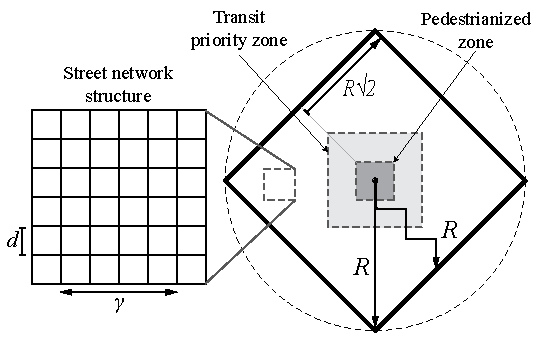
\includegraphics[width=0.5\textwidth]{diagram_pedtransit_grid_city}
     \caption{Rectilinear city with pedestrianized corridor}
     \label{fig:gridcity}
\end{figure}

\noindent The objective is to model the traffic impact on the surrounding street network in order to determine:
\begin{enumerate}[topsep=3pt, itemsep=3pt, partopsep=3pt, parsep=3pt]
    \itshape
    \item what are the optimal pedestrian and transit zone sizes?
    \item what are the impacts on travel time?
    \item what are the resulting shifts in demand?
\end{enumerate}

\section{Demand}
Demand is generated in the city area in units of $\frac{trips}{dist^2 \cdot time}$, and can be simplified into two types:

\begin{itemize}
    \item uniform baseline travel across the network, $\lambda_b$, and 
    \item monocentric travel demand going to and from the center of the city, $\lambda_c$. 
\end{itemize}

The baseline traffic flows associated with average trip length $l$ generate $q_b = \frac{\lambda_b l}{\delta}$ flow across the network. The average distance for baseline and monocentric trips in a rectilinear city are $l_b=\frac{14}{15}R$ and $l_c=\frac{2}{3}R$, respectively; with an overall average travel distance of $\bar{l} = \frac{r(14\lambda_b + 10\lambda_c)}{15(\lambda_b + \lambda_c)}$. The additional traffic flow associated with trips to and from the center varies with the distance from the center. Consider a narrow square of infinitesimal width $dr$ at radius $r$ from the center. The total demand for trips crossing this square is $2\lambda_m (R^2 - r^2)$. Each of these vehicles travels a distance $dr$ within the square, and the amount of road infrastructure is $8r\delta$ as oriented perpendicular (as shown), or $4\sqrt{2}r\delta$ as a 45-degree diamond. $\delta$ is the density of available road network in $\frac{lane \cdot dist}{dist^2}$. The calculation for network density is derived as the total roadway length $2n(n+1)d$, divided by total area $nd^2$; both of which can be expressed as a function of the number of city blocks $n$, and the street spacing dimension $d$. Since the function is linearly constant, of $\delta$ with respect to $d$, yielding $\delta = \frac{2}{d}$.

The flow across the network at a point $r$ distance from the city center is then calculated as the combined sum of the baseline demand and the monocentric demand, calculated as:

\begin{equation}
    q_a(r) = \frac{14R\lambda_b}{15\delta} + \frac{\lambda_c}{4\delta r} \left(R^2 - r^2 \right)
    \label{eq:flowacross}
\end{equation}


The pedestrianized zone will cause some trips to be diverted around the perimeter zone. Trips can be categorized into four distinct types (see Figure~\ref{fig:diverted}):

\begin{enumerate}
	\item Unimodal routes entirely within the pedestrianized zone that are unaffected by the zone, 
	\item Unimodal routes entirely outside the pedestrianized zone that are unaffected by the zone,
	\item Bimodal routes taking vehicles around the perimeter of the pedestrianized zone to park nearest the destination and the remaining radial distance is traveled on foot,
	\item Unimodal routes that would have passed through the center travels around the perimeter of the pedestrianized zone vertically and horizontally, and
	\item Unimodal routes that would have passed through the center travels around the perimeter of the pedestrianized zone diagonally.
\end{enumerate}

\begin{figure}[!ht]
     \centering
     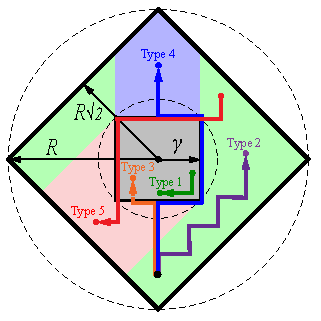
\includegraphics[width=0.3\textwidth]{diagram_diverted_routes}
     \caption{Diverted route types}
     \label{fig:diverted}
\end{figure}


The flow around the perimeter road is then calculated as the sum of the flow generated by the four trip types:

\begin{subequations}
\begin{align}
	q_1(\gamma) &= 0 \\
	q_2(\gamma) &= \left[2 \lambda_b \left(R^2 - \gamma^2\right) \times \frac{\gamma^2}{R^2} \times\frac{\gamma}{2}\right] \frac{4d}{8\gamma (R-2)}\\
	q_3(\gamma) &= \left[2 \lambda_b \left(R^2 - \gamma^2\right) \times \frac{\gamma (2R - 3\gamma)}{2R^2} \times  3\gamma\right] \frac{4d}{8\gamma (R-2)}\\
	q_4(\gamma) &= \left[2 \lambda_b \left(R^2 - \gamma^2\right) \times \frac{\gamma (\sqrt{2}R-\gamma)}{R^2} \times  3\gamma\right] \frac{4d}{8\gamma (R-2)}\\
\end{align}
\end{subequations}

\noindent which can be simplified to:

\begin{align}
	    q_p(\gamma) & = \sum\limits_{i=1}^4 q_i(\gamma) = \frac{2\lambda_b \gamma \left(6R(1+\sqrt{2}) - 11\gamma\right) \left(R^2 - \gamma^2\right)}{\delta R^2(R-2)}
    \label{eq:perimflow}
\end{align}


\noindent The flow across the network at distance $r$ from the center from the function in Equation~\eqref{eq:flowacross} possesses the form shown in Figure~\ref{fig:flowacross}, and flow around the perimeter of the pedestrian zone from the function in Equation~\eqref{eq:perimflow} possesses the form shown in Figure~\ref{fig:perimflow}. As the distance from the city increases, traffic decreases. When traffic near the center exceeds capacity, one might consider simply pedestrianizing the city center out to the point where capacity if first exceeded. However, as the pedestrian zone size increases so does traffic on the perimeter road. 

\begin{figure}[!ht]
     \centering
     \hfill
     \begin{subfigure}[b]{0.45\textwidth}
         \centering
         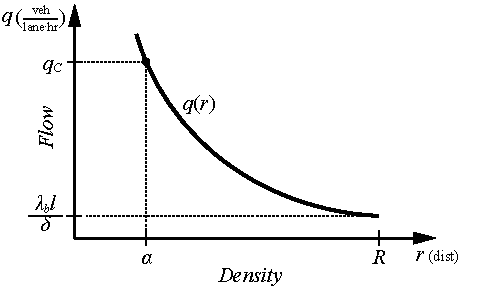
\includegraphics[width=\textwidth]{diagram_flow_across}
         \caption{Trip demand flow at point $r$ distance from center}
         \label{fig:flowacross}
     \end{subfigure}
     \hfill
     \begin{subfigure}[b]{0.45\textwidth}
         \centering
         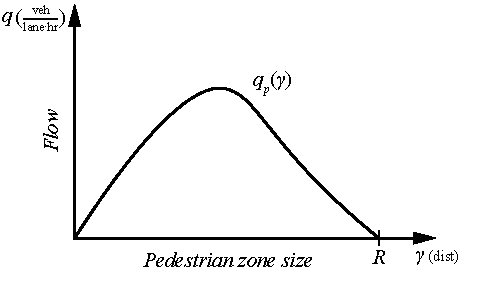
\includegraphics[width=\textwidth]{diagram_flow_perim}
         \caption{Trip demand flow on perimeter of pedestrian zone}
         \label{fig:perimflow}
     \end{subfigure}
     \hfill
     \caption{Macroscopic fundamental diagram and travel time cost function}
\end{figure}

\section{Traffic flow}
Traffic flow through the network is characterized by the macroscopic fundamental diagram (see Figure~\ref{fig:mfd}) as a function of density. A travel time function (see Figure~\ref{fig:traveltime}) then depends upon the state of traffic flow through the network as being either ``uncongested'' (solid line) or ``congested'' (dashed line) in Figures~\ref{fig:mfd} and~\ref{fig:traveltime}.

\begin{figure}[!ht]
     \centering
     \hfill
     \begin{subfigure}[b]{0.45\textwidth}
         \centering
         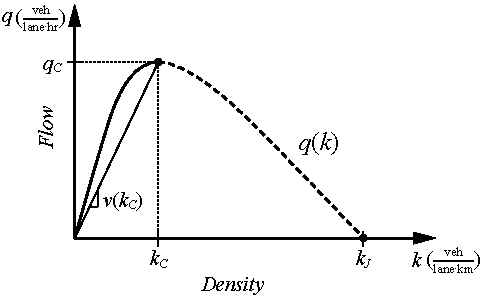
\includegraphics[width=\textwidth]{diagram_mfd}
         \caption{Macroscopic fundamental diagram}
         \label{fig:mfd}
     \end{subfigure}
     \hfill
     \begin{subfigure}[b]{0.45\textwidth}
         \centering
         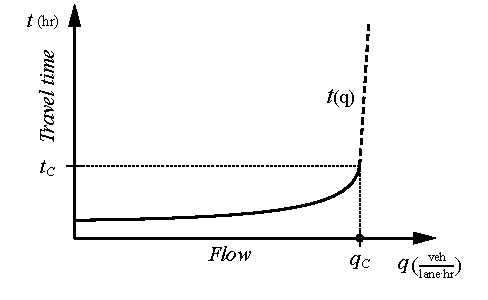
\includegraphics[width=\textwidth]{diagram_traveltime}
        \caption{Travel time cost function}
         \label{fig:traveltime}
     \end{subfigure}
     \hfill
     \caption{Macroscopic fundamental diagram and travel time cost function}
\end{figure}

Assuming for this case a parabolic function for the uncongested portion of the flow-density relationship, an expression for the ``uncongested'' solid line porition of Figure~\ref{fig:mfd} can be written as:

\begin{equation}
    q(k) = q_{c} - \frac{\left(k-k_{c}\right)^{2}}{\alpha_0} = q_{c}\frac{k\left(2k_{c}-k\right)}{k_{c}^{2}}
\end{equation}

\noindent where $k_c$ is the density at capacity, $q_c$ is the flow at capacity, and $\alpha_0 = \frac{k_c^2}{q_c}$ is the parameter used to center the left side of the parabola at the origin. In order to determine travel time using density as a function of flow $k(q)$, which can be solved for using the quadratic formula:

\begin{equation}
    k(q) = k_{c}-\sqrt{\alpha_0\left(q_{c}-q\right)} = k_c \left(1 - \sqrt{1- \frac{q}{q_c}} \right)
    \label{eq:densityparabolic}
\end{equation}

\noindent A piecewise monotonic cost function for travel time can then be defined as:
\begin{subequations}
\begin{align}
    t_D(q) &= l \frac{k(q)}{q} & \text{for}~q < q_c \\
    t_D(q) &= t_c \left(\frac{q}{q_c}\right)^{20} = l\frac{k_c}{q_c} \left(\frac{q}{q_c}\right)^{20} & \text{for}~q \geq q_c
\end{align}
\end{subequations}

\noindent where $t(q)$ is travel time for flow $q$, $k(q)$ is traffic density for flow $q$, $l$ is link length, $q_c$ is link capacity, and $t_c = l\frac{k_c}{q_c}$ is the travel time at capacity. The average travel time in traffic $\bar{t}$, can be determined from the average travel distance $\bar{l}$, divided by average speed $\bar{v}$:

\begin{equation}
    \bar{t} = \frac{\bar{l}}{\bar{v}} = \bar{l}~\frac{k\left(\bar{q_a}\right)}{\bar{q_a}}
\end{equation}

\noindent which can be analytically determined from the MFD as a function of average flow across the network $\bar{q_a}$, as experienced by travelers from their trips between the pedestrian zone $\gamma$, to the city limit $R$:

\begin{align}
    \bar{q}_a & = \frac{1}{R-\gamma}\int_\gamma^R q(\gamma) d\gamma \notag\\
    \bar{q}_a & = \frac{14R\lambda_{b}}{15\delta} +  \frac{\lambda_{c}}{8\delta (R - \gamma)} \left[ 2R^{2} ln \left( \frac{R}{\gamma}\right) + \gamma^{2} - R^{2}\right]
\end{align}

\section{Transit}

Transit travel time is conditional upon whether it operates in a transit priority zone (e.g., dedicated lane or right-of-way) or in mixed-traffic (e.g., city bus). In assuming no other source of delay in a transit priority zone, the travel time of transit is then

\begin{subequations}
\begin{align}
    t_{TP} & = \frac{l}{v_{m}} + \frac{l}{s}t_s  & \text{with transit priority} \\
    t_{TM}(q) & = l\frac{k(q)}{q} + \frac{l}{s}t_s  & \text{without transit priority when}~q < q_c\\
    t_{TM}(q) & = l\frac{k_c}{q_c} \left(\frac{q}{q_c}\right)^{20} + \frac{l}{s}t_s & \text{without transit priority when}~q \geq q_c
\end{align}
\end{subequations}

\noindent where $v_m$ is the maximum cruising speed of transit unimpeded by traffic, $s$ is stop spacing, and $t_s$ is stop time. The stop time is essentially the lost time inclusive of acceleration, deceleration and dwell time. The travel time of transit in mixed-traffic will then always be higher than driving an automobile, eventually converging as traffic conditions reach jam flow. Transit priority provides a constant travel time which will be initially slower than driving in uncongested traffic conditions, but will eventually reach a traffic flow point $q^*_T$, where the travel time of transit with priority exceeds driving (see Figure~\ref{fig:transittraveltime}).

\begin{figure}[!ht]
     \centering
     \hfill
     \begin{subfigure}[b]{0.45\textwidth}
         \centering
         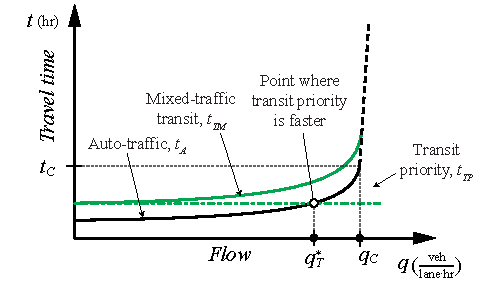
\includegraphics[width=\textwidth]{diagram_transit_traveltime}
        \caption{Transit travel time}
         \label{fig:transittraveltime}
     \end{subfigure}
     \hfill
     \begin{subfigure}[b]{0.45\textwidth}
         \centering
         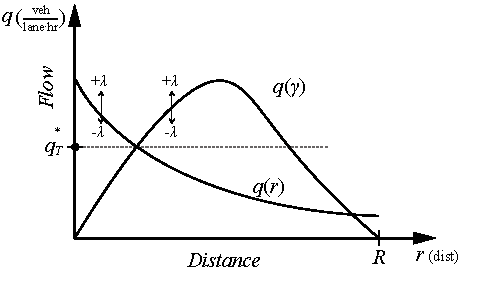
\includegraphics[width=\textwidth]{diagram_flow_combo}
         \caption{Optimal pedestrian and transit priority zone size}
         \label{fig:flowcombo}
     \end{subfigure}
     \hfill
     \caption{Transit travel time and optimal zone sizing}
\end{figure}

The critical transit priority traffic flow point $q^*_T$, is found where transit priority travel time $t_{TP}$ intersects driving travel time $t_D$. Since travel time is a piece-wise function, it depends on whether the transit priority travel time $t_{TP}$, exceeds the driving travel time at roadway capacity $t_c$. Although it is unlikely that transit priority travel time will exceed traffic travel time, the condition is provided nonetheless. To determine when this occurs, a simple ratio can be taken, $\sfrac{t_{TP}}{t_c} = \frac{q_c}{k_c} \left( \frac{1}{v_m} + \frac{t_s}{s} \right)$. The critical transit priority traffic flow point then depends on whenther $\sfrac{t_{TP}}{t_c}$ is greater than or less than 1:

\begin{subequations}
\begin{align}
    q^*_T & = \frac{2k_{c}}{T} - \frac{k_{c}^{2}}{q_{c}T^{2}} & \text{for}~ \sfrac{t_{TP}}{t_c} < 1 \\
    q^*_T & = q_{c}\left(\frac{q_{c}}{k_{c}}T\right)^{\frac{1}{20}} & \text{for}~ \sfrac{t_{TP}}{t_c} \geq 1 \\
    \text{where: } & T = \frac{1}{v_{m}} + \frac{t_{s}}{s} \notag
    \end{align}
\end{subequations}

\noindent 


$q^*_T$ could then be used in combination with network flow at distance $r$ in Equation~\eqref{eq:flowacross} to determine the optimal transit priority zone, $\tau^*$. The solution to this is quadratic, but assuming a non-negative value for the optimal transit zone size, it can be solved for analytically:

\begin{equation}
    \tau^* = \frac{56\lambda_{b}-60\delta q_{t} +\sqrt{\left(56\lambda_{b}-60\delta q_{t}\right)^{2}+900\lambda_{c}^{2}R^{2}}}{30\lambda_{c}}
\end{equation}

Determining an optimal pedestrian zone size is slightly more complex. An appropriate pedestrian zone size can exist anywhere in the range $q_a(\gamma) < q_c > q_p(\gamma)$ where the pedestrian zone is (see Figure~\ref{fig:flowcombo}):

\begin{enumerate}[label=(\alph*)]
    \item large enough to prevent traffic flow across the network from exceeding capacity $q_a(\gamma) < q_c$, and 
    \item small enough to prevent perimeter traffic flow from exceeding capacity $q_p(\gamma) < q_c$. 
\end{enumerate}

The intersection point of the two functions may be used as an optimal compromise, ensuring both conditions are satisfied with the least possible traffic flow. However, setting $q_a = q_p$ to find the intersection point results in a quintic function (polynomial to the $5^{th}$ power):

\begin{equation}
f(\gamma) = \frac{11}{R^{2}}\gamma^{5}-\frac{6(1+\sqrt{2})}{R}\gamma^{4}-11\gamma^{3}+\frac{48\lambda_{b}R(1+\sqrt{2})+\lambda_{c}(R-2)}{8\lambda_{b}}\gamma^{2}-\frac{14R(R-2)}{30}\gamma-\frac{\lambda_{c}R^{2}(R-2)}{8\lambda_{b}}
\end{equation}

\noindent yielding multiple points where the function is equal to zero (see Figure~\ref{fig:optimalped}) and cannot be easily solved analytically.

\begin{figure}[!ht]
     \centering
     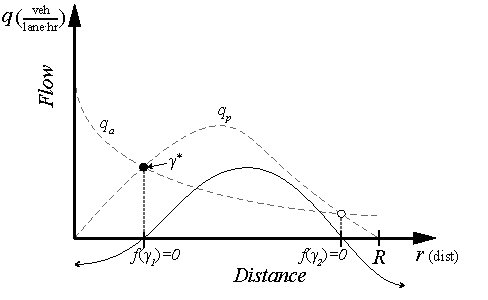
\includegraphics[width=0.5\textwidth]{diagram_optimalped}
     \caption{Quintic function for optimal pedestrian zone size, $f(\gamma)$}
     \label{fig:optimalped}
\end{figure}

Given that the pedestrian zone size must exist between $0 \leq \gamma \leq R$ an optimal pedestrian zone dimension $\gamma^*$, can be found numerically. Since two intersection points between $q_a$ and $q_p$ exist, the minimum of the two provides the desired optimal $\gamma^*$:

\begin{align}\small
\gamma^* &\Leftarrow \text{min} \left[ f(\gamma_1) = 0, f(\gamma_2) = 0 \right]\\
\text{s.t.} & ~ 0 \leq \gamma \leq R 
\end{align}

\section{Distance traveled}
To determine the travel time, the total average distance traveled must be calculated for the following modes:

\begin{description}
    \item [Bicycle and pedestrian] trips are also generated by the baseline demand (b) and the monocentric central demand (c). Let $D_{ij}$ be demand amount and $l_{ij}$ be the average walking distance covered in each case $ij$ where $i$ is trip types $\{1,3\}$ and $j$ is demand type $\{b,c\}$. The total distance covered by foot or bike $L_W$ is then:

\begin{equation}
     L_W = \frac{ D_{1b}l_{1b} + D_{1c}l_{1c} + D_{3b}l_{3b} + D_{3c}l_{3c} } { D_{1b} + D_{1c} + D_{3b} + D_{3c} }
\end{equation}

where: 
\begin{itemize}
    \item $D_{1b} = 2 \lambda_b \gamma^2 \times \frac{\gamma^2}{R^2}$ : Total baseline demand trips originating in pedestrian zone by the proportion ending in the pedestrian zone.
    \item $D_{3b} = 4 \lambda_b (R^2 - \gamma^2) \times \frac{\gamma^2}{R^2}$ : Total baseline demand trips originating inside and ending outside the pedestrian zone, and vice versa. Both cases equal $2\lambda_b (R^2 - \gamma^2) \times \frac{\gamma^2}{R^2}$.
    \item $D_{1c} = 2 \lambda_c \gamma^2$ : Total monocentric demand trips originating inside the pedestrian zone.
    \item $D_{3c} = 2 \lambda_c (R^2 - \gamma^2)$ : Total monocentric demand trips originating outside the pedestrian zone.
    \item $l_{1b} = \frac{4}{3}\gamma$ : Average distance of baseline trips with uniformly distributed origins and destinations.
    \item $l_{3b} = \frac{5}{3}\gamma$ : Average distance from uniformly distributed point on the pedestrian zone perimeter to some uniformly distributed destination in the zone.
    \item $l_{1c} = \gamma$ : Average distance of monocentric trips ending at the center with uniformly distributed origins.
    \item $l_{3c} = \gamma$ : Average distance from pedestrian zone perimeter to center.
\end{itemize}

The combined function then becomes:

% \begin{equation}
% L_W = \frac{8\lambda_b \gamma^5 + 20\lambda_b \gamma^3 (R^2-\gamma^2)}{3R^2} + 2\lambda_c \gamma^3 + 2\gamma (R^2 - \gamma^2)
% \end{equation}

\begin{equation}
L_W = \frac{R^{2}\gamma^{3}\left(10\lambda_{b}+3\lambda_{c}-3\right)-6\lambda_{b}\gamma^{5}+3R^{4}\gamma}{3R^{2}\gamma^{2}\left(2\lambda_{b}+\lambda_{c}-1\right)-3\lambda_{b}\gamma^{4}+3R^{4}}
\end{equation}





\item[Driving] distance is the average driving distance for baseline trips ($\frac{14}{15}(R-\gamma)\times\frac{\lambda_b}{\lambda_b + \lambda_c}$) and monocentric trips ($\frac{2}{3}(R-\gamma)\times\frac{\lambda_c}{\lambda_b + \lambda_c}$) outside of the pedestrian zone, multiplied by the proportion of respective trip demand. The combined function can be simplified to

\begin{equation}
L_D = \frac{(R-\gamma)(14\lambda_b + 10\lambda_c)}{15(\lambda_b + \lambda_c)}
\end{equation}

\item[Transit] distance must be separated by the portion traveled in transit priority and in mixed traffic to calculate the appropriate travel time:

\begin{itemize}
    \item In mixed traffic it is the average distance traveled outside the priority zone:
    
    \begin{equation}
        L_{TM} = \frac{(R-\tau)(14\lambda_b + 10\lambda_c)}{15(\lambda_b + \lambda_c)}
    \end{equation}
        
    \item In transit priority it is the average distance traveled inside the priority zone:
    
    \begin{equation}
        L_{TP} = \frac{\tau (14\lambda_b + 10\lambda_c)}{15(\lambda_b + \lambda_c)}
    \end{equation}
    
\end{itemize}

\end{description}

\section{Mode choice}
Assuming unlimited transit capacity relative to driving and that transit priority is unaffected by congestion, a transit system with transit priority in this model effectively serves as a pressure release for demand. As congestion increases with driving trips, transit becomes more appealing, thus drawing trips away from driving. Conversely, a reduction in congestion would attract trips towards driving as the driving travel time has improved. Assuming transit provides a reasonable and reliable alternative to driving, some demand equilibrium exists where the travel time cost of driving matches transit. The mode choice can be modeled as the probability of choosing to drive $P_D$ or transit $P_T$, using a simple two-alternative logit model with (dis-)utility as the choice travel cost:

\begin{subequations}
    \label{eq:choiceprob}
    \begin{align}
        P_D & = \frac{1}{1+e^{- (\beta_D t_D-t_T \beta_T)}}\\
        P_T & = 1 - P_D
    \end{align}
\end{subequations}

\noindent where $t_D$ and $t_T$ are the travel times associated with automobile and transit, respectively; and $\beta$ is the a estimated scaling parameter. The probability in Equation~\eqref{eq:choiceprob} can be used to find the proportion of trips made by driving. A two-alternative logit can be simplified to require only the utility difference between the two choices, not the full value, thus the logit only requires a travel time differential $\Delta t = t_D - t_T$:

\begin{equation}
    \Delta t(q) = \beta_D\overset{drive}{\left[ L_D \frac{k(q)}{q} + \frac{L_D}{v_{walk}} \right]} - \beta_T \overset{transit}{\left[ \left( \frac{L_{TP}}{v_{max}} + \frac{L_{TP}}{s}t_s \right) + \left( L_{TM} \frac{k(q)}{q} + \frac{L_{TM}}{s}t_s \right) \right]}
\end{equation}

The new demand is then shifted according to the proportional mode choice probability $P_D$ for baseline and monocentric demand $\hat{\lambda_b} = P_D \lambda_b$, and monocentric demand $\hat{\lambda_c} = P_D \lambda_c$. As travel time will vary depending upon $\tau$ and $\gamma$, there is some sort of dynamic equilibrium with flow and demand where travel time depends on flow and flow depends on travel time. 



\end{document}
